\documentclass{article}

\usepackage{frongillo}

\title{\textbf{Orale di italiano\\Corso Passerella}}
\author{Matteo Frongillo, Paolo Bettelini}

\begin{document}

\maketitle
\tableofcontents
\phantom{}
\pagebreak


%%%%%%%%%%%%%%%
\paragraph*{Suddivisione testi}

\textbf{Paolo}
\begin{itemize}
    \item Dante Alighieri (Oltre la spera, Inferno I, Inferno III);
    \item Machiavelli (Sintesi della vita di Machiavelli, Lettera al Vettori, Dedica, Capitoli I, VI, XV, XVIII, XXV);
    \item Ariosto (Vita di Ariosto con personaggi esterni [Ippolito, Alessandra, Boiardo] , Canti I, XIX, XXIII)
    \item Pietro Verri (Spiegare l'illuminismo e il Caffé, Lettera agli amici milanesi);
    \item Beccaria (Capitoli I, VI, XII).
\end{itemize}

\textbf{Matteo}
\begin{itemize}
    \item Petrarca (Struttura di Rvf, vita di Petrarca, Capitoli I, III, XVI, XXII, XC, CCCX);
    \item Boccaccio (Struttura del Decameron, Peste, Novelle II.5, III.2, IV.5, V.8, VI.10, VII.1);
    \item Leopardi (Spiego l'illuminismo e il pessimismo, Islandese, Venditore d'almanacchi, L'Infinito, La quiete dopo la tempesta, Sabato del villaggio).
\end{itemize}

%%%%%%%%%%%%

\newpage
\part{Esami scritti}

\section{Come analizzare in base all'autore}
\textbf{Dante}
\begin{itemize}
    \item Passo di un canto della \textit{Commedia} o prosimetro della \textit{Vita nova};
    \item Seguire il testo dalla lettera al concetto;
    \item Fare analogie con gli altri canti.
\end{itemize}

\textbf{Boccaccio}
\begin{itemize}
    \item Novella del \textit{Decameron};
    \item Seguire tutto il testo passo passo;
    \item Analisi a livelli:
        \begin{itemize}
            \item Analisi dei personaggi;
            \item Analisi degli spazi e dei tempi se necessario;
        \end{itemize}
    \item Arrivare al sistema di valori che sta dietro alla novella;
    \item Fare attenzione alla struttura del testo:
        \begin{itemize}
            \item Rubrica;
            \item Cornice;
            \item Coordinata ideologica spesso relativa ad altre novelle;
        \end{itemize}
    \item Fare analogie con le altre novelle.
\end{itemize}

\textbf{Petrarca}
\begin{itemize}
    \item Canto del \textit{Rerum vulgarium fragmenta};
    \item Spiegare di cosa parla il testo;
    \item Analisi:
        \begin{itemize}
            \item Analizzare strofa per strofa;
            \item Analizzare il testo dal generale allo specifico;
            \item ``Essere / dover essere'' 
        \end{itemize}
    \item Ritornare dall'analisi di ogni strofa al generale di tutto il testo:
        \begin{itemize}
            \item Capire come è strutturato il testo;
            \item Cercare figure retoriche nella struttura:
                \begin{itemize}
                    \item Struttura fatta a climax;
                    \item Struttura fatta a similitudine (``ma'' avversativo);
                \end{itemize}
        \end{itemize}
    \item Dare importanza alle analogie tra i verbi;
    \item Dare importanza all'utilizzo dei diversi tempi verbali.
\end{itemize}

\textbf{Machiavelli}
\begin{itemize}
    \item Capitolo de \textit{Il Principe};
    \item Seguire il testo durante l'analisi;
    \item Ripetere sostanzialmente ciò che dice l'autore, concentrandosi sugli snodi cruciali;
    \item Tenere in considerazione la vita politica di Machiavelli e il suo ruolo importante
        come consigliere;
    \item Riallacciare i discorsi alla sua vita e agli altri testi leggi;
    \item Citare il testo (per gli scritti).
\end{itemize}

\textbf{Beccaria e Verri}
\begin{itemize}
    \item Capitolo di \textit{Dei delitti e delle pene};
    \item Seguire il testo durante l'analisi;
    \item Ripetere sostanzialmente ciò che dice l'autore, concentrandosi sugli snodi cruciali;
    \item Tenere in considerazione la vita di Beccaria e il ruolo de \textit{Il Caffé};
    \item Riallacciare i discorsi alla sua vita e agli altri testi leggi;
    \item Citare il testo (per gli scritti).

\end{itemize}

\textbf{Ariosto}
\begin{itemize}
    \item Passo di un canto dell'\textit{Orlando furioso};
    \item Parlare in generale di cosa tratta il passo;
    \item Analizzare ogni ottava dal generale allo specifico;
    \item Correlare il passo agli altri canti letti.
\end{itemize}

\textbf{Leopardi}
\begin{itemize}
    \item Canto di \textit{Canti} oppure opera delle \textit{Operette morali};
    \item Trattare i temi legati alla ragione della vita, pessimismo e Natura impersonificata;
    \item Riflessioni sulla vita;
    \item Analisi accompagnata da passi dello \textit{Zibaldone};
    \item Correlare il canto o l'opera alle altre viste e ai passi dello \textit{Zibaldone}.
\end{itemize}

%%%%%%%%%%%%

\newpage

\part{Esame Orale}

\section{Dante Alighieri}

\subsection{Vita nova}

\begin{enumerate}
    \item Vita nova è il primo prosimetro di Dante
    \item Racconta la storia d'amore di Dante per Beatrice;
    \item Questa vicenda diventa un modello per questa tipologia di narrativa
    \item Il titolo indica come Dante consideri l’inizio della sua vita (nuova vita, rinnovata) quando
    vide Beatrice per la prima volta.
    \item Il primo contatto amoroso nella poesie è spesso caratterizzato da un
    innamoramento a prima vista.
    \item Quando la voce dell’interesse di Dante nei confronti di Beatrice le giunge, lei gli nega il saluto.
    \item Il saluto nel medioevo ha un significato molto più profondo di quello odierno.
    \item Nonostante il rifiuto, Dante continua ad esprimere il suo amore verso Beatrice semplicemente lodandola
    (scrivendo di lei), completamente senza ricambio di interesse
    \item Questa loda rappresenta la forma più pura di amore.
    \item Questo libro introduce la simbologia del numero 9 associato a Beatrice. Ciò è dato dal fatto che Dante
    l’abbia vista per la prima volta a 9 anni, rivista 9 anni dopo, e altri motivi che vengono descritti. Il numero
    9 è anche un simbolo biblico (3 volte la trinità).
\end{enumerate}

\subsubsection{Oltre la spera che più larga gira}

\begin{enumerate}
    \item È l'ultimo sonetto di Vita nova, il libro che racconta la storia d'amore di Dante
    per Beatrice.
    \item È importante considerare il significato del titolo di Vita nova (vedi prima).
    \item Questo sonetto descrive il concetto di intelligenza nova indotta nello spirito di Dante.
    \item Il primo verso è una perifrasi che indica “oltre il corpo celeste più lontano” (chiamato Il Primo Mobile), ossia il
    paradiso siccome la visione dell’universo era quella tolemaica e creazionista.
    \item Per contestualizzare è necessario parlare del sistema tolemaico (di Claudio Tolomeo), ossia il sistema geocentrico.
    \item Secondo questo sistema, la terra è fissa al centro degli universo (elemento antropocentrista)
    \item Attorno, I vari pianeti ruotano attorno alla terra in delle orbite circolari sempre più distanti
    \item Questi corpi celesti sono trascinati da delle sfere di cristallo (ossia un manteriale perfetto, indistruttibile).
    \item Queste credenze derivano dalla Genesi, il primo libro della Bibbia, che descrive la creazione del mondo da parte di Dio in sei giorni.
    \item Dalla descrizione del firmamento della bibbia, ossia quello di essere come una cupola, nasce l'idea di sfere di cristallo che sostengono i corpi celesti.
    \item Il Primo Mobile rappresenta quindi la sfera più esterna dell'universo, che contiene tutte le stelle fisse.
    \item oltre il Primo Mobile, vi è il paradiso con Dio. Ed è proprio questo al quale Dante sta facendo riferimento (oltre l'ultima sfera)
    \item Il secondo verso ci indica che il sospiro del poeta esce dal suo cuore, mentre è vivo, dalla sua intimità più
    profonda, e attraverso i cieli fino al paradiso.
    \item Ai versi 3-4 viene descritto ciò che permette questo percorso, ossia ciò che lo tira verso l’alto.
    \item Questa forza è un’intelligenza nova, ossia una nuova sensibilità nel vedere le cose.
    \item Questa nuova intelligenza deriva dall’amore, che permette all’autore di avere una nuova consapevolezza.
    \item L'sperienza amorosa è dolorosama porta ad una nuova capacità di intendimento. 
    \item Amore personificato con la A maiuscola, classico elemento del dolce Stilnovo.
    \item La seconda quartina descrive il punto di arrivo.
    \item Quando lo spirito arriva, vede una donna, la quale viene
    onorata dagli altri beati, Dio e la Madonna.
    \item Viene anche detto che questa donna brilla (luce è un verbo).
    \item causa di questo grande splendore, lo spirito giunto in paradiso (pellegrino, in pellegrinaggio) la ammira.
    \item Dalla terza quartina Lo spirito ripercorre il medesimo tragitto verticale, ma al contrario, tornando da Dante.
    \item Questo spirito cerca di spiegargli che cosa ha visto. “La vede tale che quando me lo ridice, io non capisco”
    \item Dante non comprende
    quindi ciò che lo spirito gli riferisce, perché “parla sottile”, ossia parla in maniera troppo difficile.
    \item Il cuore dolente del poeta è ciò che fa sì che lo spirito venga interrogato.
    \item Infatti, lo spirito parla proprio al cuore \underline{e} a
    Dante (questo amplifica l’incomprensione della spiegazione)
    \item Lo spirito parla in maniera troppo complessa
    perché il linguaggio non riesce ad esprimere quello che si è provato (topos dell’ineffabilità, è ineffabile) siccome
    l’esperienza lo trascende.
    \item Alla quarta terzina Dante capisce che la donna in questione è Beatrice nonostante l'incomprensione con il suo spirito.
    \item Nella poesia antica, la parola gentile è molto più profonda di quella odierna e possiede un significato diverso, ossia un significato nobile di purezza (nobiltà d'animo).
    \item La parola ``però'' vuol dire ``per ciò''. 
    \item Beatrice viene nominata, una occasione molto rara.
    \item Infinite, l'ultimo verso è dato dal fatto che Dante si stesse riferendo a delle Donne nel testo, quindi non è rilevante.
    \item Nel complesso, il sonetto è diviso in due. Vengono distinte le due verticalità del viaggio, avanti e indietro.
    \item Molte parole della prima parte appartengono alla sfera visiva, poiché il paradiso è fatto di luci
    \item Molte parole della seconda parte riguardando dal sfera del parlare.
    \item Per cui lo spirito può vedere ma ha l'impossibilità di esprimersi.
    \item Questa separazione è collegata dall'uso di due parole quasi uguali, \textbf{mira} e \textbf{Vedela} (detto per anadiplosi).
\end{enumerate}

\newpage
\subsection{La Commedia}
\subsubsection{Inferno I}

--

\newpage
\subsection{La Commedia}
\subsubsection{Inferno III}

--

\newpage
\section{Francesco Petrarca}
\subsection{Rerum vulgarium fragmenta}
\subsubsection{I}

--

\newpage
\subsubsection{III}

--

\newpage
\subsubsection{XVI}

--

\newpage
\subsubsection{XXII}

--

\newpage
\subsubsection{XC}

--

\newpage
\subsubsection{CCCX}

--

\newpage
\section{Giovanni Boccaccio}
\subsection{Decameron}
\begin{enumerate}
    \item L'opera è stata scritta a Firenze durante l'epidemia di peste nera del 1348;
    \item È strutturata con una cornice narrativa e cento novelle.
    \item Cornice narrativa:
    \begin{enumerate}[label*=3.\arabic*.]
        \item La cornice narrativa segue un gruppo di dieci giovani fiorentini aristocratici,
            composto da sette donne e tre uomini, che si rifugiano nella campagna toscana per
            sfuggire alla peste;
        \item Il gruppo soggiornerà per quattordici giorni nella villa in campagna;
        \item Per passare il tempo, ciascuno di loro racconta una novella al giorno, per un
            totale di cento novelle in dieci giorni;
        \item I giorni di racconto sono dieci poiché i fine settimana sono dedicati all'igiene
            personale e alla preghiera;
        \item Ogni giorno viene eletto a turno un re o una regina tra i dieci giovani che
            avrà il compito di stabilire il tema della giornata, sul quale le novelle narrate
            dovranno basarsi;
        \item I temi delle giornate variano tra l'\textbf{amore}, la \textbf{fortuna} e 
            l'\textbf{ingegno}; 
    \end{enumerate}
    \item Novelle:
        \begin{enumerate}[label*=\arabic*.]
            \item Le novelle spaziano in temi e argomenti come:
            \begin{itemize}
                \item La vita;
                \item L'amore;
                \item L'umorismo;
                \item L'ingiustizia sociale;
                \item La morale;
                \item La religione;
                \item La società medievale;
            \end{itemize}
        \item Ogni giornata contiene dieci novelle, per un totale di cento narrate nel corso
            dei dieci giorni;
        \item Le novelle sono scritte in prosa e sono basate su esperienze umane;
        \end{enumerate}
    \item Conclusione:
        \begin{enumerate}[label*=\arabic*.]
            \item L'opera si conclude con una breve riflessione di Boccaccio, il quale
                sottolinea l'importanza dell'amicizia, dell'amore e della sorte nella vita
                umana;
            \item Boccaccio riconosce il potere della narrazione come mezzo per affrontare le
                difficoltà e per trovare conforto e compagnia;
            \item Morale che nonostante le difficoltà, la vita continua e la bellezza e la
                gioia possono ancora essere ritrovate.
        \end{enumerate}
\end{enumerate}

\newpage
\subsubsection{Introduzione alla Prima giornata}
\textbf{Proemio}
\begin{enumerate}
    \item Dedica alle donne (Paragrafi 1-7):
        \begin{enumerate}[label*=\arabic*.]
            \item Boccaccio si rivolge direttamente alle donne, giustificando l'inizio
                dell'opera con una riflessione sulla necessità di passare attraverso la
                sofferenza prima di arrivare al piacere;
            \item L'autore si scusa con le donne lettrici poiché l'introduzione, pur dolorosa,
                è essenziale per comprendere il contesto in cui si sviluppano le novelle;
            \item La sofferenza amorosa e il desiderio di offrire conforto alle donne sono
                i temi centrali dei paragrafi;
        \end{enumerate}
\end{enumerate}
\textbf{Giornata prima - Introduzione}    
\begin{enumerate}
    \item L'arrivo della peste a Firenze (Paragrafi 8-13):
        \begin{enumerate}[label*=\arabic*.]
            \item La narrazione del Decameron inizia con l'arrivo della peste nera a Firenze;
            \item L'origine della peste, dicendo che ha avuto origine in
                Oriente e che è arrivata in Europa attraverso le rotte commerciali e tramite
                i topi infetti sulle navi mercantili;
            \item La peste è vista come una possibile punizione divina per i peccati degli
                uomini;
            \item Vengono descritti i sintomi della malattia: gonfiore, febbre alta,
                eruzioni cutanee e sangue da naso che portavano inevitabilmente alla morte;
            \item Boccaccio parla dell'impotenza dei medici e delle cure del tempo contro una
                malattia così contagiosa che colpiva indistintamente uomini e animali;
        \end{enumerate}
    \item Reazioni della popolazione alla peste (Paragrafi 19-23):
        \begin{enumerate}[label*=\arabic*.]
            \item Alcune persone scelgono di vivere moderatamente ma con vitto raffinato e di
                alta qualità;
            \item Altre decidono di abbandonarsi agli eccessi, facendo festa e concedendosi
                ogni piacere;
            \item La gente vede la disgregazione delle leggi divine e umane e la distruzione
                delle strutture sociali e morali;
        \end{enumerate}
    \item Pampinea propone di lasciare Firenze (Paragrafi 53-65):
        \begin{enumerate}[label*=\arabic*.]
            \item Pampinea propone alle altre sei conoscenti di abbandonare Firenze per
                cercare rifugio nella campagna;
            \item Sottolinea che questa non è una scelta di disimpegno, ma un necessità di
                preservare la propria onestà e dignità in un contesto pericoloso;
            \item L'obiettivo è vivere una vita onesta e serena in campagna, lontano dalla
                decadenza della città, mantenendo un equilibrio tra divertimento e ragione;
        \end{enumerate}
    \item Organizzazione del viaggio (Paragrafi 67-78)
        \begin{enumerate}[label*=\arabic*.]
            \item La campagna viene descritta con le caratteristiche di un ``locus amoenus'',
                esattamente in contrapposizione alla città di Firenze in quel periodo, la
                quale presentava vicoli e case molto strette e le strade ricoperte di cadaveri;
            \item La fuga dalla città non è definitiva, ma è una temporanea ricerca di pace e
                sicurezza;
            \item Filomena e Elissa discutono sulla necessità di avere degli uomini nel gruppo
                per garantire sicurezza e guida, poiché un gruppo di donne donne veniva
                considerata di natura litigiosa e paurosa, secondo i pregiudizi dell'epoca;
        \end{enumerate}
    \item Inclusione dei tre uomini (Paragrafi 78-81)
        \begin{enumerate}[label*=\arabic*.]
            \item Coincidenza vuole che tre giovani uomini (Panfilo, Filostrato e Dioneo),
                innamorati di alcune delle ragazze, entrino nella chiesa dove le donne si
                erano ritrovate per assistere alla messa;
            \item I tre uomini sono di buone maniere e nobili, come le donne, e vengono
                inclusi nel gruppo per bilanciare e guidare il gruppo;
        \end{enumerate}
    \item Trasferimento alla villa (Paragrafi 88-89)
        \begin{enumerate}[label*=\arabic*.]
            \item Pampinea approccia i ragazzi e insieme organizzano il trasferimento dalla
                città alla campagna;
            \item Il luogo scelto è una villa a due miglia da Firenze, descritta come un
                palazzo con sale affrescate, cortili, logge, giardini meravigliosi e cantine
                di vini raffinati;
        \end{enumerate}
    \item Proposta di incoronare re o regina giornalmente (Paragrafi 88-90)
        \begin{enumerate}[label*=\arabic*.]
            \item Dioneo esprime il desiderio di lasciarsi alle spalle i pensieri tristi della
                città, proponendo di cantare e divertisti sempre nei limiti dell'onestà;
            \item Pampinea propone una rotazione giornaliera di leadership, per mantenere
                l'ordine nel gruppo e per eliminare ogni forma di esclusione e favoritismo;
            \item Il primo re viene scelto collettivamente, mentre i successivi vengono
                nominati dai predecessori.
        \end{enumerate}
\end{enumerate}

\newpage
\subsubsection{II, 5 (Andreuccio da Perugia)}
\begin{enumerate}
    \item Riassunto generale della novella:
        \begin{enumerate}[label*=\arabic*.]
            \item \textbf{Rubrica:} si trova nella seconda giornata ed è raccontata da
                Fiammetta;
            \item \textbf{Giornata:} la giornata è dedicata alle avventure e alle disavventure
                a lieto fine;
            \item \textbf{Tema:} il tema centrale è la creascita personale attraverso
                l'esperienza, rappresentata dalle tre cadute e risalite di Andreuccio;
            \item \textbf{Cornice:} non fa parte della novella;
            \item \textbf{Coordinata ideologica:} la storia riflette l'idea che l'ingegno e
                l'adattabilità sono essenziali per superare le difficoltà e prosperare;
        \end{enumerate}
    \item Struttura: è suddiviso in tre paragrafi (tre incidenti):
        \begin{enumerate}[label*=\arabic*.]
            \item Chiassetto: vialetto tra le case dove Andreuccio cade per la
                prima volta;
            \item Pozzo: luogo della seconda caduta, che rappresenta una discesa più
                profonda e pericolosa;
            \item Arca: la discesa nell'arca è il momento più rischioso e simbolico
                della novella;
        \end{enumerate}
        In tutte e tre i luoghi dell'incidente c'è una caduta, ossia una discesa, più o meno
        volontaria, da un luogo più alto a uno più basso. In ogni incidente la risalita dopo
        la caduta è sempre più difficile da affrontare, ma la riuscita indica un punto di
        maturazione di Andreuccio.
    \item Descrizione dei personaggi:
        \begin{enumerate}[label*=\arabic*.]
            \item \textbf{Andreuccio da Perugia:}\\
                inizialmente inesperto, ingenuo e vanitoso. Attraverso le disavventure
                sviluppa capacità critica e ingegno e si arricchisce monetariamente;
            \item \textbf{Fiordaliso:}\\
                scaltra, furba e ingegnosa, non si avvicina direttamente ad Andreuccio quando
                lui mostra i soldi, ma pianifica il suo inganno con astuzia, ottima
                commediante e finta vittima, crea un'illusione di nobiltà e si è preparata con
                dettagli su Andreuccio per manipolarlo;
            \item \textbf{Altri personaggi (Buttafuoco, la vecchia e i due ladri):}\\
                antagonisti che rappresentano degli ostacoli, ognuno dei quali contribuisce a
                creare situazioni di pericolo e inganno che Andreuccio deve superare;
        \end{enumerate}
    \item Tempo e spazio:
        \begin{enumerate}[label*=\arabic*.]
            \item Il tempo è unitario: tutte le tre avventure avvengono in una notte;
            \item Lo spazio è una struttura circolare: Si allontana da Perugia e torna a
                Perugia;
            \item Alternanza tra luoghi aperti e chiusi:\\
                Albergo (C), Mercato (A), Casa di Fiordaliso (C), Vie di Napoli (A),
                Baracca (C), Pozzo (A), Chiesa (C);
            \item Ogni luogo rappresenta una tappa significativa nel percorso di crescita
                di Andreuccio;
        \end{enumerate}
    \item Realità storica:
        \begin{enumerate}[label*=\arabic*.]
            \item Napoli di notte era una città insicura. Questo rifletteva già una realtà
                storica nel `300;
            \item Il commercio dei cavalli a Napoli era molto fiorente all'epoca;
            \item Molte persone sono emigrate dalla Sicilia verso Napoli per la battaglia dei
                Vespri; 
            \item Tutti i personaggi e i luoghi sono realmente esistiti;
        \end{enumerate}
    \item Novella letteraria:
        \begin{enumerate}[label*=\arabic*.]
            \item La novella ha dei tratti fiabeschi:
                \begin{itemize}
                    \item Allontanamento da casa -- si impara -- si torna a casa;
                    \item Personaggio con diversi antagonisti che lo mettono alla prova;
                    \item Riesce a superare le prove con un lieto fine; 
                \end{itemize}
            \item La novella ha dei tratti di romanzo di formazione:
                \begin{itemize}
                    \item Il protagonista è maturato dopo le numerose esperienze;
                    \item Andreuccio cresce, diventando più scaltro, ingegnoso e più ricco.
                \end{itemize}
        \end{enumerate}
    \item Sistema di valori e interpretazione storico-ideologica:
        \begin{enumerate}[label*=\arabic*.]
            \item La novella parla dell'importanza dell'esperienza come strumento di crescita
                personale;
            \item Andreuccio ha una crescita diventando più furbo e scaltro, ma finalizzata
                sulla base dei beni materiali, ragionando come un mercante;
            \item Boccaccio fa una riflessione sul comportamento mercantile: chi sa cavarsela
                e utilizzare l'ingegno riesce ad arricchirsi;
            \item Tutti i personaggi con scopo di arricchirsi materialmente riescono nel loro
                scopo;
            \item Boccaccio non ha nessun giudizio morale su cosa possa comportare il peccato
                di furto nella vita eterna, bensì gli interessa chi riesce a cavarsela
                sfruttando l'ingegno a suo favore per la vita terrena;
        \end{enumerate}
\end{enumerate}

\newpage
\subsubsection{III, 2 (Lo stalliere del re Agilulf)}
\begin{enumerate}
    \item Riassunto generale della novella:
        \begin{subenumerate}
            \item \textbf{Rubrica:} la novella racconta di come lo stalliere del re Agilulf
                riesca ad ingannare il re e la regina attraverso il suo ingegno;
            \item \textbf{Giornata:} terza giornata, raccontata da Pampinea, dedicata alle
                storie di chi, grazie alla propria prontezza d'ingegno, riesce a ottenere
                ciò che desidera o a salvarsi da una situazione pericolosa;
            \item \textbf{Tema:} il tema centrale è l'ingegno e la capacità di salvarsi
                attraverso l'astuzia e prontezza;
            \item \textbf{Cornice (paragrafi 1-3):}
                \begin{subenumerate}
                    \item §1: si parla di come hanno reagito alla novella precendente e al
                        fatto che la regina dia la parola a Pampinea;
                    \item §2: è una massima di Pampinea (coordinata ideologica);
                    \item §3: Pampinea inizia la novella, dimostrando la coordinata ideologica
                        appena esposta;
                \end{subenumerate}
            \item \textbf{Coordinata ideologica:} c'è gente che vuole già sapere tutto, ma
                questo potrebbe risultare controproducente, dunque alcune volte è più saggio
                non sapere;
        \end{subenumerate}
    \item Struttura del testo:
        \begin{subenumerate}
            \item La novella è principalmente divisa in due parti, entrambe con duplice beffa:
                \begin{itemize}
                    \item Obiettivo erotico;
                    \item Salvarsi dalla beffa precedente;
                \end{itemize}
            \item L'obiettivo viene raggiunto in ambedue le parti tramite un doppio scambio di
                identità con due simulazioni d'ingegno;
            \item Lo scopo delle simulazioni d'ingegno è cammuffarsi:
                \begin{itemize}
                    \item Nella prima parte, lo Stalliere simula di essere il re;
                    \item Nella seconda parte, si cammuffa tra le persone tagliando i capelli
                        a tutti con il suo stesso taglio per non farsi scoprire dal re;
                \end{itemize}
        \end{subenumerate}
    \item Personaggi:
        \begin{subenumerate}
        \item Descrizione dei personaggi:
            \begin{subenumerate}
                \item \textbf{Re Agilulf:} uomo di grande virtù e senno, calmo e riflessivo,
                    dimostrando ingegno e autocontrollo nell'affrontare il presunto tradimento
                    della moglie, riconoscendo il valore dell'astuzia dello stalliere;
                \item \textbf{Regina:} bellissima, saggia e onesta, ma vittima delle
                    circostanze che la sendono sospettabile di infedeltà;
                \item \textbf{Stalliere:} di vilissima condizione ma di bell'aspetto, mostra
                    grande osservazione e pianificazione, capacità di rimanere calmo e di non
                    vantarsi del suo successo; 
            \end{subenumerate}
        \item Analisi del rapporto tra i personaggi:
            \begin{subenumerate}
                \item Si tratta di un triangolo amoroso, con la donna cantata al vertice
                    più alto e i due uomini sullo stesso piano in basso;
                    \begin{center}
                        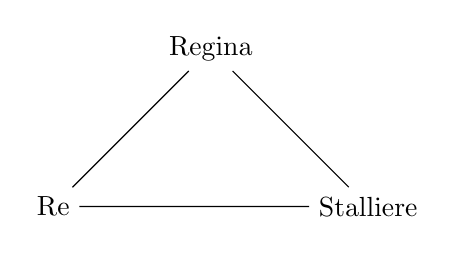
\begin{tikzpicture}
                            \node (A) at (0, 2) {Regina};
                            \node (B) at (-2, 0) {Re};
                            \node (C) at (2, 0) {Stalliere};
                            \draw (A) -- (B) -- (C) -- (A);
                        \end{tikzpicture}
                    \end{center}
                \item La donna cantata è sempre messa socialmente al vertice più alto;
                \item Amore unidirezionale che, pur non corrisposto, nobilita chi lo prova;
                \item Più la speranza diminuisce e più il desiderio cresce, il quale,
                    diventando insostenibile, porterebbe al suicidio di chi lo prova pur
                    di non soffrire più di desiderio;
                \item Lo stalliere si innamora con animo nobile;
                \item Il re e lo stalliere si trovano allo stesso piano sia sull'ambito
                    dell'ingegno, sia sul piano erotico, nonostante socialmente siano opposti;
            \end{subenumerate}
        \end{subenumerate}
    \item Sistema di valori:
        \begin{subenumerate}
            \item Nobiltà d'animo vs. ingegno:
                \begin{subenumerate}
                    \item La nobiltà d'animo è un valore cavalleresco, rappresentato dal re
                        e dalla regina;
                    \item L'ingegno è un valore borghese, rappresentato dallo stalliere, che
                        sovverte la sua condizione sociale attraverso l'astuzia;
                \end{subenumerate}
            \item Tutti e tre i personaggi guadagno da questa storia:
                \begin{subenumerate}
                    \item Lo stalliere e la regina hanno avuto una notte indimenticabile;
                    \item Il re ha convinto la regina che lui sia in grado di saperla
                        soddisfare;
                \end{subenumerate}
            \item La novella mette in luce la possibilità di sovvertire le gerarchie sociali
                attraverso l'intelligenza e l'inganno, ponendo così una tensione tra i due
                temi della nobiltà e dell'ingegno che riflette i cambiamenti sociali
                dell'epoca, con l'emergere della borghesia e dei nuovi valori legati
                all'abilità personale.
        \end{subenumerate}
\end{enumerate}

\newpage
\subsubsection{IV, 5 (Lisabetta da Messina)}
\begin{enumerate}
    \item Struttura:
        \begin{subenumerate}
            \item Premessa [§3]: Parte della cornice. Parla Filomena, la quale,
                riallacciandosi alla novella precedente di Elissa, premette che quella che
                racconterà lei non sarà una novella che tratterà di ``genti di sì alta
                condizione'', ma ciononostante non sarà meno dolorosa di quella di Elissa.
            \item Antefatto [§§4-5]:
                \begin{subenumerate}
                    \item Filomena inizia a narrare di cosa tratterà la storia;
                    \item Parla di tre fratelli mercanti a Messina, arricchiti con i soldi
                        dell'eredità del padre, con la loro sorella Lisabetta, non ancora
                        maritata;
                    \item Introduce il garzone pisano Lorenzo, che iniziò a piacere a
                        Lisabetta e, con amore corrisposto, erano diventati inseparabili
                        in anima e corpo;
                \end{subenumerate}
            \item Svolgimento dell'azione:
                \begin{subenumerate}
                    \item Protagonisti: fratelli [§§6-23]:
                        \begin{itemize}
                            \item Scoperta della tresca [§§6-7]: i fratelli di Lisabetta
                                scoprono la relazione segreta tra lei e Lorenzo;
                            \item Omicidio [§§8-9]: i fratelli uccidono Lorenzo per
                                salvaguardare l'onore della famiglia;
                            \item Domande di Lisabetta [§§10-11]: Lisabetta chiede ai suoi
                                fratelli di Lorenzo, ma riceve risposte evasive;
                        \end{itemize}
                    \item Protagonista: Lisabetta [§§11-18]:
                        \begin{itemize}
                            \item Sogno [§§12-13]: Lisabetta sogna Lorenzo che le rivela il
                                luogo della sua sepoltura;
                            \item Scoperta del cadavere e recupero della testa [§§14-16]:
                                Lisabetta si reca nel luogo indicato nel sogno, scava e
                                trova il corpo di Lorenzo, prendendo con sé la sua testa;
                            \item Culto per il vaso [§§17-18]: Lisabetta pianta la testa
                                di Lorenzo in un vaso di basilico, che cura con devozione;
                        \end{itemize}
                    \item Protagonisti: fratelli [§§19-22]:
                        \begin{itemize}
                            \item Sottrazione del vaso: i fratelli, sospettosi del
                                comportamento di Lisabetta, le sottraggono il vaso di
                                basilico e scoprono la testa di Lorenzo;
                        \end{itemize}
                    \item Protagonista: Lisabetta [§23]:
                        \begin{itemize}
                            \item Morte: Lisabetta muore di dolore, dopo aver perso sia
                                Lorenzo sia il vaso contenente la sua testa;
                        \end{itemize}
                \end{subenumerate}
            \item Origine della novella [§§23-24]: la storia di Lisabetta di Messina è un
                racconto popolare, narrato e cantato;
        \end{subenumerate}
    \item Sistema dei personaggi:
        \begin{subenumerate}
            \item Struttura dei personaggi alternata:
                \begin{subenumerate}
                    \item Evidenzia la mancanza di scambi verbali
                    tra la sorella e i fratelli, tranne nei momenti di richiesta di
                    informazioni sulla posizione del garzone, le quali non vengono neanche
                    risposte;
                    \item Per Boccaccio, l'assenza di parole indica soggezione e timore. In
                    questo caso, Lisabetta si sente intimorita dai fratelli;
                \end{subenumerate} 
            \item I personaggi si esprimono con i fatti e non con le parole:
                \begin{subenumerate}
                    \item Fratelli (personaggi forti):
                        \begin{itemize}
                            \item Usano l'azione;
                            \item Superiori dal punto di vista patriarcali (maschi) e sociali
                                (mercanti, più importanti di garzoni e fanti);
                            \item Subordinano tutto in funzione degli affari e alla loro
                                reputazione da mercanti, ragionano su costi e benefici
                                (ragione di mercatura) [§§6,7,22];
                            {\color{gray}{\item I fratelli non sono mai nominati, privi di
                                identità individuale;
                            \item Agiscono da vigliacchi, ingannando Lorenzo, 3 contro 1,
                                colpendolo alle spalle e senza assumersi nessuna
                                responsabilità [§5];}}
                        \end{itemize}
                    \item Lisabetta (+Lorenzo, +Fante) (personaggi deboli):
                        \begin{itemize}
                            \item Espressione dei sentimenti attraverso il principato
                                [§§11,12,14,16,17,18,20,23];
                            \item Rivolge domande cariche di sentimenti ai fratelli
                                [§§10,11,13,20];
                            \item Sentimenti disinteressati e genuini, non condizionati dagli
                                affari e dal lavoro;
                            \item Personaggi condannati a una condizione di inferiorità sia
                                per ragioni di sesso sia per ceto sociale;
                        \end{itemize}
                \end{subenumerate}
            In questa novella nessuno vince, la sorella perde l'amore e muore per il dolore,
            i fratelli devono lasciare il paese e perdere tutti gli affari locali;
        \end{subenumerate}
    \item Interpretazione:
        \begin{subenumerate}
            \item Interpretazione storico-ideologica:
                \begin{itemize}
                    \item Boccaccio accusa la cecità della logica mercantile del guadagno,
                        la quale non guarda in faccia a nessuno se non agli affari,
                        colpevolizzando i fratelli per la morte della sorella per presalvare
                        i loro affari;
                    \item Lorenzo e Lisabetta non hanno un monumento del loro amore. Esso
                        viene celebrato e ricordato solo a parole e nelle canzoni [§24],
                        rendendo Lisabetta una persona sconfitta;
                    \item Confronto con \underline{Lo stalliere del re Agilulf}: mentre lo
                        stalliere dopo essersi beffato del re riesce a porsi un limite,
                        i fratelli di Lisabetta non si pongono nessun limite, arrivando
                        addirittura a compiere un omicidio e a fuggire anonimamente;
                \end{itemize}
            \item Interpretazione psicoanalitica:
                \begin{itemize}
                    \item In questa novella è più importante il linguaggio non verbale
                        piuttosto di ciò che non viene detto;
                    \item Personaggi forti e deboli:
                        \begin{itemize}
                            \item  I tre fratelli non sono in grado di: amare, comunicare,
                            fare (non hanno intraprendenza: se Lorenzo non ci fosse stato,
                            loro non avrebbero avuto le capacità di fare i loro affari) [§5];
                            \item Lisabetta è in grado di: amare, comunicare, prendere
                                iniziativa;
                            \item I fratelli sotto aspetto psicoanalitico sono personaggi
                                deboli e tristi, mentre Lisabetta e Lorenzo personaggi forti
                                e felici;
                        \end{itemize}
                    \item Sviluppo dei personaggi:
                        \begin{itemize}
                            \item I tre fratelli sono privi di identità, si conosce solo che
                                sono imparentati con Lisabetta;
                            \item I tre non sono in grado di provare le stesse emozioni della
                                sorella e questo gli causa gelosia e la non accettazione di
                                non poterle provare;
                            \item La loro vigliaccheria è confermata dalla loro maleducazione
                                nelle interazioni con la sorella e con Lorenzo, che è stato
                                ucciso con l'inganno;
                            \item Colpa e sottomissione:
                                \begin{itemize}
                                    \item Lisabetta interiorizza la colpa e accetta la
                                        violenza verbale come giusta;
                                    \item Nel sogno di Lisabetta, le accuse del garzone non
                                        sono verso i fratelli ma verso di lei. Accuse
                                        chiaramente sviluppate nella sua mente e mai dette
                                        da Lorenzo, poiché lei si crede responsabile della
                                        sua morte;
                                \end{itemize}
                        \end{itemize}
                    \item Metafora materna: inizia la distorsione della realtà e la pazzia
                        di Lisabetta:
                        \begin{itemize}
                            \item La scena dell'amputazione della testa è metaforicamente
                                legata alla scena di un parto, come se la testa fosse un
                                figlio messo in un panno e dato ``in grembo'' alla serva
                                [§15];
                            \item La testa di Lorenzo diventa un simbolo di
                                amore materno e cura, il basilico rappresenta la crescita e
                                la fertilità, che Lisabetta vede crescere rigogliosa proprio
                                come una madre vede crescere un proprio figlio [§19];
                            \item La descrizione della pianta ``divenne bellissimo e 
                                odorifero molto'' [§19] è scritta molto similmente alla
                                descrizione di Lorenzo ``esendo assai bello della persona e
                                leggiadro molto'' [§X].
                        \end{itemize}
                \end{itemize}
        \end{subenumerate}
\end{enumerate}

\newpage
\subsubsection{V, 8 (Nastagio degli Onesti)}

--

\newpage
\subsubsection{VI, 10 (Frate Cipolla)}

--

\newpage
\subsubsection{VII, 1 (Gianni Lotteringhi e la ``fantasima'')}

--

\newpage
\section{Niccolò Machiavelli}

\begin{enumerate}
    \item Niccolò Machiavelli è stato un influente pensatore, diplomatico e scrittore fiorentino 1469-1527
    \item Nato a Firenze in una famiglia di modeste origini,
    \item educazione umanistica e divenne coinvolto nella politica fiorentina
\end{enumerate}

\subsection{Modelli di comportamento: il trattato}
\subsubsection{Lettera al Vettori}

\begin{enumerate}
    \item 10 dicembre 1513 indirzzata a Francesco Vettori, una delle due opere molto famosa
    \item discute degli eventi politici dell’epoca, in particolare il suo recente licenziamento da parte dei Medici dopo la caduta della Repubblica di Firenze.
    \item è delusione per essere stato escluso dalla vita
    politica e riflette sulle difficoltà e le instabilità della politica italiana.
    \item Gli condivide le sue preoccupazioni
    sulla situazione politica del tempo e sulla necessità di un principe forte e capace per riportare l’ordine e
    la stabilità nella regione
    \item Discute anche della natura umana sottolineando la necessità per un
    governante di adattarsi alle circostanze e di essere disposto a prendere decisioni impopolari per il bene
    comune
    \item L’esilio del 1512 denota uno spartiacque.
    \item prima incontrava il re di Francia, mentre ora le
    sue giornate sono monotone e non sa cosa fare
    \item da un certo punto Machiavelli comincia a tenere
    il proprio cervello vivo studiando (leggendo): questo è il senso della sua vita, rialzando la sua scrittura.
    \item I luoghi della sua giornata sono essenzialmente tre:
    \begin{itemize}
        \item \textbf{naturali} (luoghi aperti, bosco, etc.).
            Questi luoghi sono rappresentanti delle occupazioni pratiche (caccia di uccelli, commercio, taglio legna etc.);
        \item \textbf{la strada} (luogo di riflessione e di incontro con le persone dei paesi vicini);
        \item \textbf{osteria, scrittoio} (luoghi chiusi). Questi due posti sono quasi antitetici per la loro natura.
    \end{itemize}
    \item Un ragionamento analogo può essere svolgo circa i tempi della sua giornata:
    \begin{itemize}
        \item \textbf{mattino} (occupazioni pratiche);
        \item \textbf{pomeriggio} (vita sociale);
        \item \textbf{sera e di notte} (tempo per sè, tempo dello studio).
    \end{itemize}
    \item Nella lettera vi è una incongruenza. Vengono indicati solamente i principati come argomento, quando il libro finale sarà
    più vasto. Nella lettera sembra implicare che il libro sia finito. Il libro è quindi finito o no?
    \item Inoltre dice che la dedica sarà a Giulinao de' Medici, ma in realtà lo sarà a Lorenzo il giovane.
    \item Prima descrive il libro come un ghiribizzo, quasi come un piccolo gioco, ma successivamente dice
    che può essere usato da un principe nuovo.
    \item Il dubbio dilemmatico è quello di consegnare il libro. E se darlo, darglielo personalmente o per altri
    mezzi? La lettera è quindi piena di dissirio e molto problematica.
\end{enumerate}

\newpage
\subsection{Il Principe}
\subsubsection{Dedica}

\begin{enumerate}
    \item \textbf{Introduzione alla dedica}
    \begin{enumerate}[label*=\arabic*.]
        \item Machiavelli cerca di entrare nelle grazie di un sovrano.
        \item Offre qualcosa di prezioso o gradito: \textit{la cognizione delle azioni degli uomini grandi}.
        \begin{itemize}
            \item La parola \textit{grande} indica persone di potere, senza connotazione morale.
        \end{itemize}
        \item Conoscenza acquisita da:
        \begin{itemize}
            \item Lunga esperienza delle cose moderne.
            \item Lettura dei testi antichi.
        \end{itemize}
        \item Conoscenza offerta tramite un piccolo volume: \textit{Il Principe}.
        \item Vantaggio del dono: sintesi di migliaia di pagine lette e quindici anni di esperienza.
    \end{enumerate}

    \item \textbf{Topos della modestia}
    \begin{enumerate}[label*=\arabic*.]
        \item Opposizione fra modestia e orgoglio nei testi di Machiavelli.
        \item Machiavelli minimizza l'importanza delle sue opere, pur riconoscendone la grandezza e importanza.
    \end{enumerate}

    \item \textbf{Descrizione della forma del libro}
    \begin{enumerate}[label*=\arabic*.]
        \item Esteticamente poco attraente.
        \item Machiavelli vuole che il testo venga apprezzato solo per il suo contenuto.
        \item Assenza di ornamenti per evitare che il libro venga apprezzato per altro che non sia il contenuto.
    \end{enumerate}

    \item \textbf{Giustificazione dell'autore}
    \begin{enumerate}[label*=\arabic*.]
        \item Machiavelli non vuole essere visto come presuntuoso.
        \item Paragone con pittori/cartografi:
        \begin{quote}
            \itshape
            Nè voglio sia riputata presunzione, se uno uomo di basso ed infimo stato ardisce discorrere e regolare i governi de' Principi; perchè così come coloro che disegnano i paesi, si pongono bassi nel piano a considerare la natura de' monti e de' luoghi alti, e per considerare quella de' bassi si pongono alti sopra i monti; similmente, a cognoscer bene la natura de' popoli bisogna esser Principe, ed a cognoscer bene quella de' Principi conviene essere popolare.
        \end{quote}
        \item Per parlare del popolo bisogna essere principi, per parlare dei principi bisogna essere del popolo.
        \item Questa è la motivazione di Machiavelli per scrivere il principato.
    \end{enumerate}

    \item \textbf{Conclusione della dedica}
    \begin{enumerate}[label*=\arabic*.]
        \item Machiavelli si rivolge a Lorenzo de' Medici.
        \item Gli augura il meglio nel suo potere.
        \item Sottolinea la propria posizione sfortunata.
    \end{enumerate}
\end{enumerate}

\newpage
\subsubsection{Capitolo I}

\begin{enumerate}
    \item \textbf{Introduzione}
    \begin{enumerate}[label*=\arabic*.]
        \item Citazione iniziale:
        \begin{quote}
            \itshape
            Tutti gli Stati, tutti i dominii che hanno avuto, e hanno imperio sopra gli uomini, sono stati e sono o Repubbliche o Principati.
        \end{quote}
        \item Differenza tra repubblica e principato.
        \begin{itemize}
            \item Repubblica: più democratica e partecipativa.
            \item Principato: incentrato su una singola persona o gruppo di persone. XXX
        \end{itemize}
    \end{enumerate}

    \item \textbf{Tipologie di Principati}
    \begin{enumerate}[label*=\arabic*.]
        \item Principati nuovi e ereditari.
        \begin{itemize}
            \item Principati nuovi:
            \begin{itemize}
                \item Completamente nuovi (es. Milano a Francesco Sforza).
                \item Aggiunti ad una conquista (es. Regno di Napoli al Re di Spagna).
            \end{itemize}
            \item Principati ereditari: governati da una lunga discendenza.
        \end{itemize}
        \item Citazione di esempi storici per i principati nuovi aggiunti a una conquista.
    \end{enumerate}

    \item \textbf{Termine tecnico: \textit{acquista}}
    \begin{enumerate}[label*=\arabic*.]
        \item Significato specifico di \textit{acquista} in Machiavelli: conquistare.
    \end{enumerate}

    \item \textbf{Metodi di conquista dei popoli}
    \begin{enumerate}[label*=\arabic*.]
        \item Popoli abituati alla libertà vs. popoli abituati al dominio di un principe.
        \item Conquista tramite:
        \begin{itemize}
            \item Armi d'altri (mercenari, prestate o comprate).
            \item Proprio esercito di milizia.
        \end{itemize}
    \end{enumerate}

    \item \textbf{Fortuna e virtù nella conquista}
    \begin{enumerate}[label*=\arabic*.]
        \item Conquista per fortuna: ciò che sfugge al calcolo umano.
        \item Conquista per virtù:
        \begin{itemize}
            \item Capacità tecniche del principe.
            \item Virtù come abilità, non connotazione morale.
        \end{itemize}
        \item Il principe virtuoso possiede capacità tecniche, non necessariamente qualità morali come saggezza e onestà.
    \end{enumerate}
\end{enumerate}

\newpage
\subsubsection{Capitolo VI}

\begin{enumerate}
    \item \textbf{Introduzione}
    \begin{enumerate}[label*=\arabic*.]
        \item Citazione iniziale:
        \begin{quote}
            \itshape
            De' Principati nuovi, che con le proprie armi e virtù si acquistano.
        \end{quote}
        \item Concetto di imitazione:
        \begin{itemize}
            \item Importanza di ispirarsi a modelli altissimi.
            \item Analogía dell'arciere: mirare più in alto per raggiungere il bersaglio.
        \end{itemize}
    \end{enumerate}

    \item \textbf{Modelli da imitare}
    \begin{enumerate}[label*=\arabic*.]
        \item Personaggi indicati da Machiavelli:
        \begin{itemize}
            \item \textit{Moisè}: legislatore e fondatore del popolo ebraico di Israele.
            \item \textit{Ciro II}: fondatore della monarchia di Persia.
            \item \textit{Romolo}: personaggio legato al mito della fondazione di Roma.
            \item \textit{Teseo}: re mitologico di Atene.
        \end{itemize}
        \item Caratteristiche comuni:
        \begin{itemize}
            \item Fondatori di regni o repubbliche.
            \item Successo dovuto alle proprie capacità, non alla fortuna.
            \item Difficile riconoscimento iniziale e nessuna agevolazione.
        \end{itemize}
        \item Distinzione di Machiavelli:
        \begin{itemize}
            \item Unico personaggio realmente esistito: Ciro.
            \item Moisè aveva il privilegio di parlare con Dio.
        \end{itemize}
    \end{enumerate}

    \item \textbf{Virtù e fortuna nella conquista}
    \begin{enumerate}
        \item Virtù:
        \begin{itemize}
            \item Fatica per raggiungere la carica, ma mantenimento semplice.
        \end{itemize}
        \item Fortuna:
        \begin{itemize}
            \item Guadagno della carica semplice, ma fatica nel mantenerla.
        \end{itemize}
        \item Occasione come elemento intermedio tra virtù e fortuna.
        \begin{itemize}
            \item La virtù permette di riconoscere e sfruttare l'occasione.
            \item Minima fortuna necessaria, ma grande virtù può compensare l'assenza di fortuna.
        \end{itemize}
    \end{enumerate}

    \item \textbf{Esempi di fortuna e virtù nei modelli}
    \begin{itemize}
        \item \textit{Moisè}: trovò il popolo di Israele schiavo e oppresso in Egitto.
        \item \textit{Ciro}: trovò i Persiani malcontenti.
        \item \textit{Romolo}: fu allontanato dal suo paese natale.
        \item \textit{Teseo}: trovò una popolazione dispersa e la riunì.
    \end{itemize}

    \item \textbf{Sostenitori del vecchio e nuovo regime}
    \begin{enumerate}[label*=\arabic*.]
        \item Maggiore aggressività dei sostenitori del vecchio regime, che lottano per certezze.
        \item Tiepidezza dei sostenitori del nuovo regime, che lottano per un'idea.
        \item Necessità di convinzioni forti per una lotta efficace.
    \end{enumerate}

    \item \textbf{Autosufficienza del principe}
    \begin{enumerate}[label*=\arabic*.]
        \item Autosufficienza essenziale per il successo del principe.
        \item Necessità di forza armata per mantenere il potere.
    \end{enumerate}

    \item \textbf{Convinzioni del popolo}
    \begin{enumerate}[label*=\arabic*.]
        \item Facilità di convincere il popolo, difficoltà di fargli cambiare idea.
        \item Uso delle armi per cambiare le convinzioni radicate.
    \end{enumerate}

    \item \textbf{Esempio di Ierone (Gerone) Siracusano}
    \begin{enumerate}[label*=\arabic*.]
        \item Diventò principe di Siracusa senza esperienza di potere, con l'occasione data dalla fortuna.
        \item Eliminò il vecchio esercito per crearne uno proprio e fedele.
        \item Cambiò alleanze e governò facilmente su fondamenta solide.
    \end{enumerate}
\end{enumerate}

\newpage
\subsubsection{Capitolo XV}

\begin{enumerate}[label*=\arabic*.]
    \item Introduzione al Capitolo XV:
    \begin{enumerate}[label*=\alph*.]
        \item Argomento principale del capitolo: il comportamento del principe verso sudditi e amici.
        \item Machiavelli inserisce il suo lavoro nella tradizione politica.
        \item Novità di Machiavelli: distacco dagli approcci tradizionali.
        \item Scopo dell'autore: utilità pratica dei principi.
        \item Utilizzo della verità effettiva anziché dell'immaginazione.
    \end{enumerate}
    
    \item Descrizione del Principe Perfetto:
    \begin{enumerate}[label*=\alph*.]
        \item Critica ai principi utopici basati sull'idealizzazione.
        \item Discrepanza tra realtà effettiva e immaginazione utopica.
        \item L'autore sostiene che il comportamento morale può portare alla perdita di potere.
        \item Descrizione delle virtù e dei vizi associati al principe.
    \end{enumerate}
    
    \item Ruolo dei Vizi:
    \begin{enumerate}[label*=\alph*.]
        \item Accettazione dei vizi se necessari per il bene dello stato.
        \item Giustificazione delle azioni basata sull'utilità politica anziché sulla morale.
        \item Passaggio dai valori assoluti ai valori relativi.
        \item Concetto di lealtà e sveltezza come termini neutri.
    \end{enumerate}
\end{enumerate}

\newpage
\subsubsection{Capitolo XVIII}

\begin{enumerate}[label*=\arabic*.]
    \item Tema principale del Capitolo XVIII:
    \begin{enumerate}[label*=\alph*.]
        \item Discussione su lealtà, slealtà e mantenimento della parola.
        \item Contrasto tra virtù ideali e realtà effettuale.
    \end{enumerate}
    
    \item Utilizzo della Forza e della Bestialità:
    \begin{enumerate}[label*=\alph*.]
        \item Il principe deve saper utilizzare sia la legge che la forza.
        \item Analogia con l'eroe greco Achille e il centauro.
        \item Sottolineatura della debolezza dell'argomentazione mitologica.
    \end{enumerate}
    
    \item Suddivisione della Forza Bestiale:
    \begin{enumerate}[label*=\alph*.]
        \item Astuzia della volpe e forza del leone.
        \item La parola data può essere infranta per motivi di convenienza o per prevenire danni.
        \item Necessità di adattare il comportamento alle circostanze.
    \end{enumerate}
    
    \item Inganno e Manipolazione:
    \begin{enumerate}[label*=\alph*.]
        \item Il principe non deve farsi notare quando inganna.
        \item Semplicità e ingenuità degli uomini che facilita la manipolazione.
        \item Importanza dell'immagine virtuosa del principe.
    \end{enumerate}
    
    \item Giudizio basato sui Risultati:
    \begin{enumerate}[label*=\alph*.]
        \item Il principe è giudicato in base ai fini che raggiunge.
        \item La popolazione mondiale è manipolabile.
    \end{enumerate}
\end{enumerate}

\newpage
\subsubsection{Capitolo XXV}

\begin{enumerate}[label*=\arabic*.]
    \item Tema principale del Capitolo XXV:
    \begin{enumerate}[label*=\alph*.]
        \item Discussione sul ruolo della fortuna nella vita dei principi.
        \item Contrapposizione tra la percezione comune della fortuna e la visione di Machiavelli.
    \end{enumerate}
    
    \item Immagine della Fortuna:
    \begin{enumerate}[label*=\alph*.]
        \item Descrizione della fortuna come un fiume in piena.
        \item Necessità di adattare il comportamento umano agli eventi della fortuna.
        \item Assenza di difese contro la fortuna in Italia.
    \end{enumerate}
    
    \item Ruolo della Virtù:
    \begin{enumerate}[label*=\alph*.]
        \item Importanza della virtù nel resistere alla fortuna.
        \item Relazione tra azioni dei principi e felicità o infelicità.
        \item Esempi di successo e fallimento in base all'adattamento alle circostanze.
    \end{enumerate}
    
    \item Approccio consigliato:
    \begin{enumerate}[label*=\alph*.]
        \item Preferenza per l'impetuosità rispetto al rispetto.
        \item Analisi della fortuna come simile a una donna, più facilmente conquistata con audacia.
        \item Vantaggio dei giovani nell'affrontare la fortuna con audacia.
    \end{enumerate}
\end{enumerate}

\newpage
\section{Ludovico Ariosto}

\subsection{Orlando furioso}

\begin{enumerate}
    \item Celebre poeta e drammaturgo italiano del Rinascimento (1474-1533)
    \item Visse principalmente a Ferrara, dove servì sotto il patronato dei duchi d'Este.
    \item Inizialmente intraprese la carriera giuridica, ma il suo vero amore era la poesia.
    \item Fu attivo anche come diplomatico e funzionario di corte, occupando diverse posizion
\end{enumerate}

\subsubsection{Canto I (ottave 1-44)}

\begin{enumerate}
    \item I due grandi temi del libro sono: \begin{subenumerate}
        \item L'amore (ispirato alla letteratura Bretone, la quale si sviluppò in Bretagna e in altre aree celtiche, principalmente
        a partire dal IX secolo in poi. Essa comprende leggende sui Celti (popoli indoeuropei) e la storia
        mitologica delle Isole britanniche e della Bretagna, in particolar modo quelle riguardanti re Artù e i
        suoi cavalieri della Tavola Rotonda.)
        \item La guerra (ispirato alla letteratura Carolingia, uno stile di scrittura creato durante la rinascita
        carolingia, che mirava a recuperare e preservare il sapere classico, avvenuta sotto il regno di Carlo
        Magno nei secoli VIII e IX.)
    \end{subenumerate}
    \item \textbf{Prima ottava:} \begin{subenumerate}
        \item Vi è un doppio chiasmo (v. 1 donne, amori, cavalieri, armi e vv. 1-2 donne, amori, cortesie, cavalieri, armi, audaci imprese)
    \end{subenumerate}
\end{enumerate}

\newpage
\subsubsection{Canto XIX (ottave 30-42)}

--

\newpage
\subsubsection{Canto XXIII (ottave 100-136)}

--

\newpage
\section{Pietro Verri}
\subsection{Illuminismo}
\subsubsection{Lettera agli amici milanesi}

--

\newpage
\section{Cesare Beccaria}

\subsection{Il caffè}

\begin{enumerate}
    \item L'Accademia dei Pugni fu un'istituzione culturale fondata nel 1761 a Milano
    \item Il caffè fu un periodico italiano, pubblicato 1764-1766 ad opera dei fratelli Pietro e Alessandro Verri con il contributo di Beccaria e gli intellettuali che erano soliti raccogliersi all'Accademia dei pugni.
    \item Il nome caffè deriva dal luogo, ossia la bottega, da dove nascono questi testi dell'illuminismo lombardo.
\end{enumerate}

\subsection{Dei delitti e delle pene}

\begin{enumerate}
    \item È un pamphlet del 1764
    \item Affronta temi come la pena di morte senza trattarne la moralità, bensì puramente da un punto di vista pratico e utilitista.
    \item Nasce da confronti e dibattiti sulla giurisprudenza criminale
    \item Per sottrarre il libro alla censura, Pietro Verri manda il libro in Toscana per essere pubblicato (era più progressista)
    \item Viene pubblicato senza il nome dell'autore
    \item Il libro vuole rovesciare la concezione tradizionale che lascia poca distinzione fra giustizia e vendetta, come la legge del taglione.
    \item Beccaria indica la presenza delle leggi divine (peccati), di natura e le leggi dell'uomo (reati).
\end{enumerate}

\subsubsection{Capitolo I (Origine delle pene)}

\begin{enumerate}
    \item \textbf{Il contratto sociale (Russeau):}
    \begin{enumerate}
        \item In assenza di leggi, ogni individuo ha una libertà infinita.
        \item Lo sforzo che uno deve fare per proteggersi dagli altri è troppo
        \item Le leggi sono quindi un compromesso per godere di una libertà (limitata)
        \item Le leggi sono dei vincoli, delle limitazioni alla libertà, che cercano di massimizzare il rapporto fra la libertà garantita e la libertà persa.
        \item \textbf{Esempio:} è più vantaggioso perdere il diritto di uccidere, piuttosto che poter uccidere ma rischiare di essere uccisi.
        \item Così nasce la società; per convenienza.
        \item Il \textit{deposito} è precisamente ciò che si perde.
    \end{enumerate}
    \item Secondo Beccaria le persone agiscono in base ad un calcolo razionale dei loro interessi personali, compresa la valutazione delle conseguenze delle proprie azioni.
    \item Questa concezione deriva dal \textit{sensismo}, ossia l'idea che la sfera sensoriale dell'uomo sia la cognizione più basica e importante.
    \item Ne consegue che le persone sono meno inclini a commettere crimini se sanno che saranno punite in modo rapido, certo e proporzionato alla gravità del crimine commesso
    \item Una pena per essere deterrente, deve essere sempre più svantaggiosa dell'azione commessa (deve essere sensibili).
    \item La prospettiva di una pena non ci deve abbandonare mai, come una forza costante nella nostra testa che associa l'azione alla pena.
    \item Non è quindi sufficiente insegnare i valori morali, bisogna anche avere un deterrente (critica alla Chiesa e in particolare ai gesuiti).
\end{enumerate}

\newpage
\subsubsection{Capitolo VI (Proporzione fra i delitti e le pene)}

\begin{enumerate}
    \item Non tutti i delitti sono uguali, e quelli più gravi è auspicabile che vengano commessi più raramente.
    \item Più una società diventa grande e intricata, più i delitti aumentano e vi è il rischio che le pene debbano sempre essere più dure.
    \item Questi ostacoli non possono toglierti la libertà di delinquere, bensì minimizzano
    la gravità della situazione.
    \item Il criterio per stabilire la gravità di un delitto è la tutela del deposito (del patto sociale)
    \item È impossibile creare una scala di delitti discreta (come in \(\mathbb{N}\)), perché è impossibile delineare dove
    un delitto termini e ne cominci un altro, bensì deve essere per forza continua e densa (come in \(\mathbb{R}\)).
    \item Siccome ci sono infinite delitti, è quindi impossibile catalogare con precisione le pene corrispondenti.
    \item Se questo sistema non dovesse funzionare, si arriverebbe addirittura ad una situazione dove i delitti
    sono creati dalle pene
    \item \textbf{Esempio:} quando qualcuno sceglie di commettere un crimine accettandole la pena.
    \item Se la stessa pena è data a due delitti \textit{diversi}, tantovale commettere quello dei due che conviene maggiormente.
\end{enumerate}

\newpage
\subsubsection{Capitolo XII (Fine delle pene)}

\begin{enumerate}
    \item Lo scopo delle pene non è quello di torturare
    \item Lo scopo delle pene non è quello di cancellare un delitto (e ricompensare la vittima)
    \item Ciò è dato dal fatto che non vi è un legame fra la sofferenza del reo e il delito che ha commesso,
    bensì quello di \begin{subenumerate}
        \item evitare la recidiva del reo;
        \item fare da deterrente per persone nefaste.
    \end{subenumerate}
    \item Uno Stato non può agire per passione o per fanatismo, ma dev’essere moderato e oggettivo.
    \item Secondo Beccaria, la pena perfetta deve avere le seguenti tre caratteristiche:
        \begin{subenumerate}
            \item roporzionalità al delitto;
            \item deterrente agli altri;
            \item priva di violenza.
        \end{subenumerate}
    \item Questo punto è stato molto criticato dagli stessi illuministi dal momento che non vi è una sola parola a
    favore della vittima (risarcimento).
    \item Oggi i risarcimenti consistono in denaro o lavori socialmente utili, che
    risarciscono la società.
\end{enumerate}

\newpage
\section{Giacomo Leopardi}
\subsection{Operette Morali}
\subsubsection{Dialogo della Natura e di un Islandese}

--

\newpage
\subsubsection{Dialogo di un venditore d'almanacchi e di un passeggere}

--

\newpage
\subsection{Canti}
\subsubsection{L'Infinito}

--

\newpage
\subsubsection{La quiete dopo la tempesta}

--

\newpage
\subsubsection{Il sabato del villaggio}

--













































\end{document}